\documentclass[a4paper, 11pt, titlepage]{jsarticle}
\usepackage[dvipdfmx]{graphicx}
\usepackage{array}
\usepackage{array}
\usepackage{listings}
\usepackage{amsmath}
\usepackage{comment}

\title{知能情報基礎演習II \\ 要件定義と基本設計家書の作成 \\ グループ番号7 Develoop}
\author{245429H 末吉 良多 \\ 245745J 知念 拓弥 \\ 245704B 武嶋 優海}
\date{\today}

\begin{document}
\maketitle

\clearpage

\tableofcontents
%---------------------------------------------------------------------------------------------------------------------------------------------------------------------------------------------------------------------------------------------------------------------------------
\clearpage
\section{開発するアプリ名、内容、開発の背景等}
\subsection{開発するアプリ名}
Shelfie
\subsection{内容}
自分が読んだ本、買った本の写真を撮り、デジタル本棚を作る
\subsection{開発背景}
多くの人が、読書を通じて得た感動や知識の証として、読んだ本をコレクションしたいという思いを持っています。\\
しかし、特に一人暮らしの学生など、限られたスペースや予算で生活する人々にとって、物理的な本棚を充実させていくことは簡単なことではありません。

「本は好きだけれど、置き場所がないから買えない」

「思い出深い本でも、泣く泣く手放さなければならない」\\
こうした悩みを解決し、誰もが気軽に自分だけの本棚を持てるようにしたいと思い開発を始めました。

\clearpage

\subsection{ロゴ}
\begin{figure}[htbp]
\centering

\includegraphics[width=60mm] {shelfie_logo.png}
\label{fig:func}
\end{figure}

\begin{figure}[htbp]
\centering

\includegraphics[width=60mm] {shelfie_logo2.png}
\label{fig:func}
\end{figure}
%---------------------------------------------------------------------------------------------------------------------------------------------------------------------------------------------------------------------------------------------------------------------------------
\clearpage
\section{要件定義}
今回の授業で作成するアプリの要件定義表を以下に示します。本棚として使用するために最低限必要な、書籍情報の登録、検索、編集、削除、一覧表示の業務を実装します。

また、今回は開発期間が短い都合上、ユーザー機能を実装しないこととしました。本棚の情報はブラウザのキャッシュに保存することとします。

\begin{table}[htbp]
  \centering
  \begin{tabular}{|l|l|>{\centering\arraybackslash}m{4cm}|>{\centering\arraybackslash}m{5cm}|}
    \hline
    \textbf{識別子} & \textbf{業務名} & \textbf{概要} & \textbf{備考} \\
    \hline\hline
    BM01 & 書籍登録 & 書籍の情報を登録する & 表紙画像、ISBN、JANコード、タイトル、著者名、追加日 \\
    \hline
    BM02 & 書籍検索 & 書籍の情報を基に検索する & ISBN、JANコード、タイトル、著者名、タグ \\
    \hline
    BM03 & 書籍編集 & 感想・メモの登録タグ付け機能 & タグ作成 \\
    \hline
    BM04 & 書籍削除 & 書籍の情報を削除する & 一括削除 \\
    \hline
    BM05 & 書籍一覧表示 & 登録書籍を一覧表示する & 本棚表示 \\
    \hline
  \end{tabular}
  \caption{業務要件表}
  \label{tab:requirements}
\end{table}

\section{基本設計}
\subsection{機能要件表}
基本設計では、先程の業務要件表をもとに、各機能の詳細を設計しました。優先度が高い機能から順に実装していきます。次ページに、機能要件表を示します。
\begin{table}[htbp]
  \centering
  \begin{tabular}{|>{\centering\arraybackslash}m{0.9cm}|>{\centering\arraybackslash}m{0.9cm}|>{\centering\arraybackslash}m{1.3cm}|>{\centering\arraybackslash}m{1.5cm}|>{\centering\arraybackslash}m{1.8cm}|>{\centering\arraybackslash}m{1.2cm}|>{\centering\arraybackslash}m{1.3cm}|>{\centering\arraybackslash}m{1.3cm}|>{\centering\arraybackslash}m{0.3cm}|}
    \hline
    \textbf{識別子} & \textbf{機能ID} & \textbf{機能名} & \textbf{機能要件} & \textbf{入力} & \textbf{出力} & \textbf{前提条件} & \textbf{事後条件} & \textbf{優先度} \\
    \hline\hline
    BM01 & FN01 & 書籍登録 & 書籍情報登録、識別ID割り振り & 表紙画像、ISBN、JANコード、タイトル、著者名、追加日 & 表紙画像、完了メッセージ & & 表紙画像が参照できる & 高 \\
    \hline
    BM02 & FN02 & 書籍検索 & 書籍の情報を基に検索する & キーワード、著者名、タイトル、タグ、識別ID & 検索結果 & 書籍情報が登録されている & 検索結果が表示される & 中 \\
    \hline
    BM03 & FN03 & 書籍編集 & 感想・メモの登録、タグ付け機能 & 識別ID、自由記述、タグ & 更新完了メッセージ & 識別IDが存在 & 変更内容が反映される & 高 \\
    \hline
    BM04 & FN04 & 書籍削除 & 書籍情報を削除する & 識別ID & 削除完了メッセージ & 識別IDが存在 & 本棚から本の削除、登録情報が削除されている & 高 \\
    \hline
    BM05 & FN05 & 書籍一覧表示 & 登録書籍を一覧表示する & & 書籍一覧 & 書籍情報が登録されている & 本棚に登録されている書籍が一覧表示される & 高 \\
    \hline
    BM06 & FN06 & お気に入りページ表示 & 感想文の横でお気に入りのページを表示 & ページ画像 & ページ画像 & 識別IDが存在 & 感想欄にページ画像が表示される & 中 \\
    \hline
  \end{tabular}
  \caption{機能要件表}
  \label{tab:functions}
\end{table}
%---------------------------------------------------------------------------------------------------------------------------------------------------------------------------------------------------------------------------------------------------------------------------------
\clearpage
\subsection{ワイヤーフレーム}
Figmaで作成。そのスクリーンショットを添付する。

\begin{figure}[htbp]
\centering
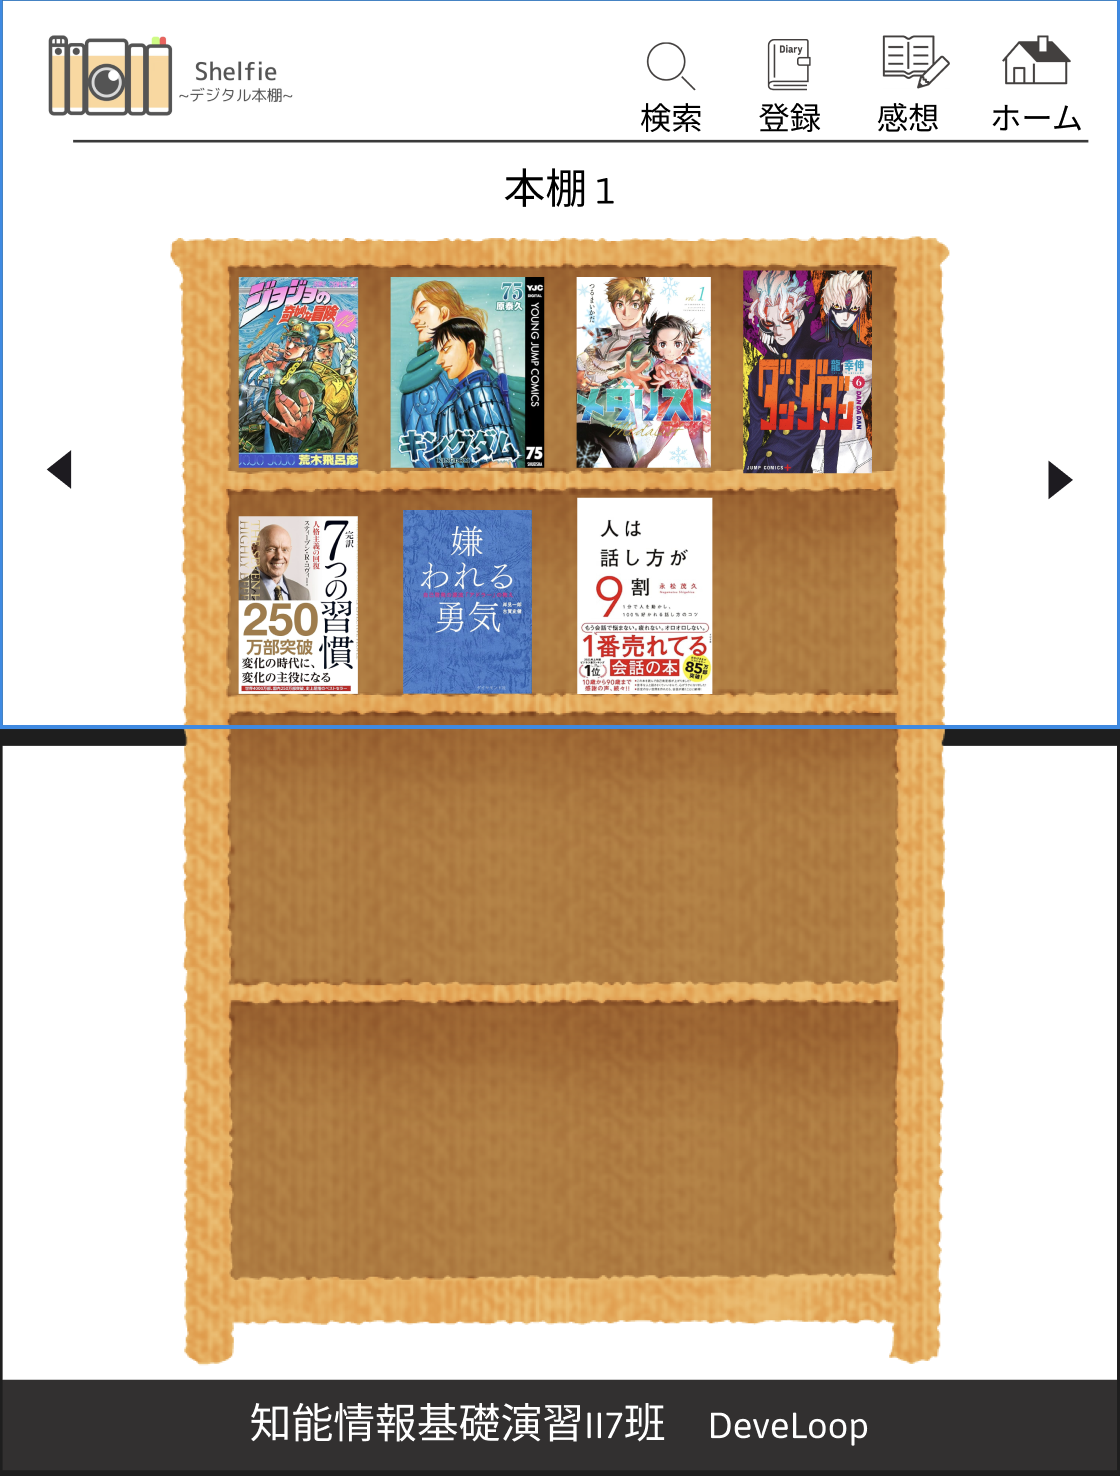
\includegraphics[width=70mm]{toppage.png}
\caption{トップページ}
\label{fig:func}
\end{figure}

トップページの画面解説
\begin{itemize}
    \item \textbf{ヘッダーメニュー:} 画面上部に配置された主要機能へのナビゲーション。
    \begin{itemize}
        \item \textbf{検索(虫眼鏡アイコン):} 登録したい本を探す機能。
        \item \textbf{登録(ペンのアイコン):} 新しい本を本棚に追加する機能。
        \item \textbf{感想(本のアイコン):} 本の感想を記録・閲覧する機能。
        \item \textbf{ホーム(家のアイコン):} メインの本棚画面に戻る機能。
    \end{itemize}

    \item \textbf{デジタル本棚:} 画面中央の、ユーザーが登録した本を可視化するエリア。
    \begin{itemize}
        \item \textbf{タイトル(本棚1):} 本棚番号の表示。
        \item \textbf{本の表紙:} 登録した本の表紙を並べる。漫画から自己啓発書まで多様なジャンルに対応。
    \end{itemize}

    \item \textbf{フッター:} 画面最下部に開発者情報を記載。
    \begin{itemize}
        \item 知能情報基盤演習1I7班 DeveLoop
    \end{itemize}
\end{itemize}
%---------------------------------------------------------------------------------------------------------------------------------------------------------------------------------------------------------------------------------------------------------------------------------
\clearpage
\begin{figure}[htbp]
\centering
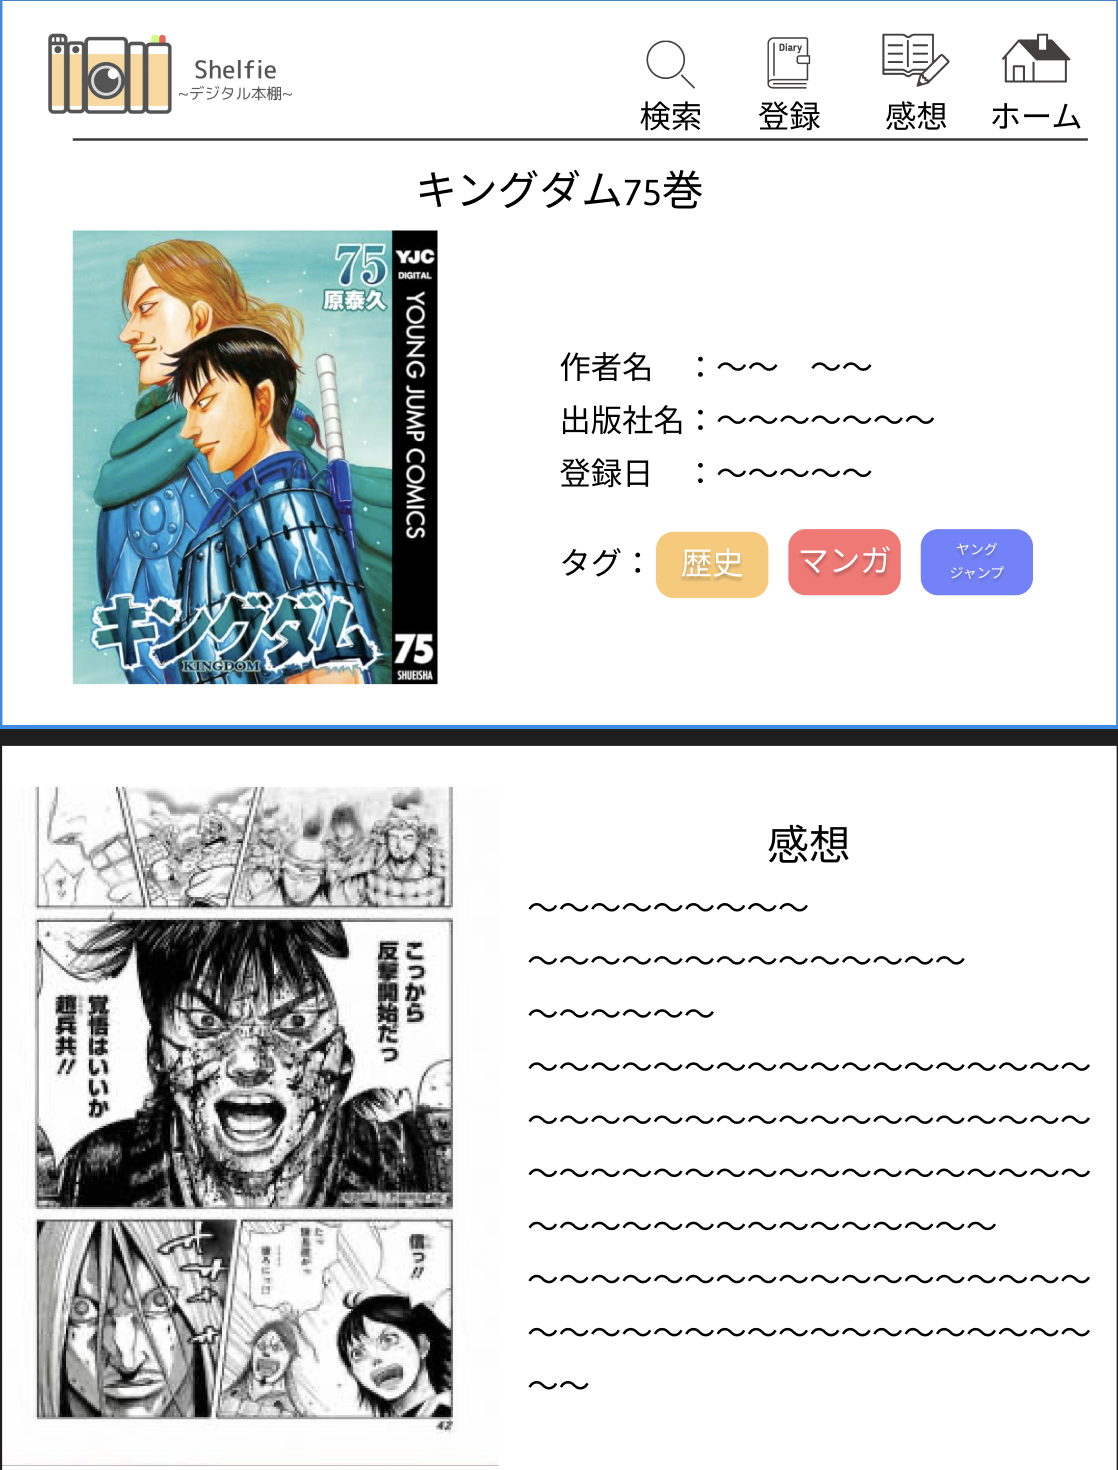
\includegraphics[width=70mm]{detailpage.png}
\caption{本の詳細ページ}
\label{fig:func}
\end{figure}

詳細ページの画面解説

\begin{itemize}
    \item \textbf{画面の概要:}
    本棚に登録した個別の書籍について、詳細情報を確認し、自身の感想を記録・閲覧するためのページ。

    \item \textbf{画面の構成要素:}
    \begin{itemize}
        \item \textbf{ヘッダーメニュー:} ホーム画面と共通のナビゲーションが配置。
        \item \textbf{書籍情報エリア:} 画面上部に配置された、選択した本のデータ領域。
        \begin{itemize}
            \item \textbf{書名・書影:} 本のタイトルと表紙画像が大きく表示される。
            \item \textbf{詳細データ:} 作者名、出版社名、登録日などのメタデータを記録する項目。
            \item \textbf{タグ:} 「歴史」「マンガ」等のタグ付けにより、ユーザー自身が本を分類・整理できる機能。
        \end{itemize}

        \item \textbf{感想エリア:} 画面下部に配置された、ユーザーの個人的な記録スペース。
        \begin{itemize}
            \item \textbf{画像挿入:} 漫画のコマなどが挿入されており、心に残ったシーンを視覚的に保存できる機能を示唆。
            \item \textbf{テキストエリア:} 自由な形式で感想文を書き込める。
        \end{itemize}
    \end{itemize}
\end{itemize}
%---------------------------------------------------------------------------------------------------------------------------------------------------------------------------------------------------------------------------------------------------------------------------------
\clearpage
\subsection{ユースケース}
MIROで作成。そのスクリーンショットを添付する
\begin{figure}[htbp]
\centering
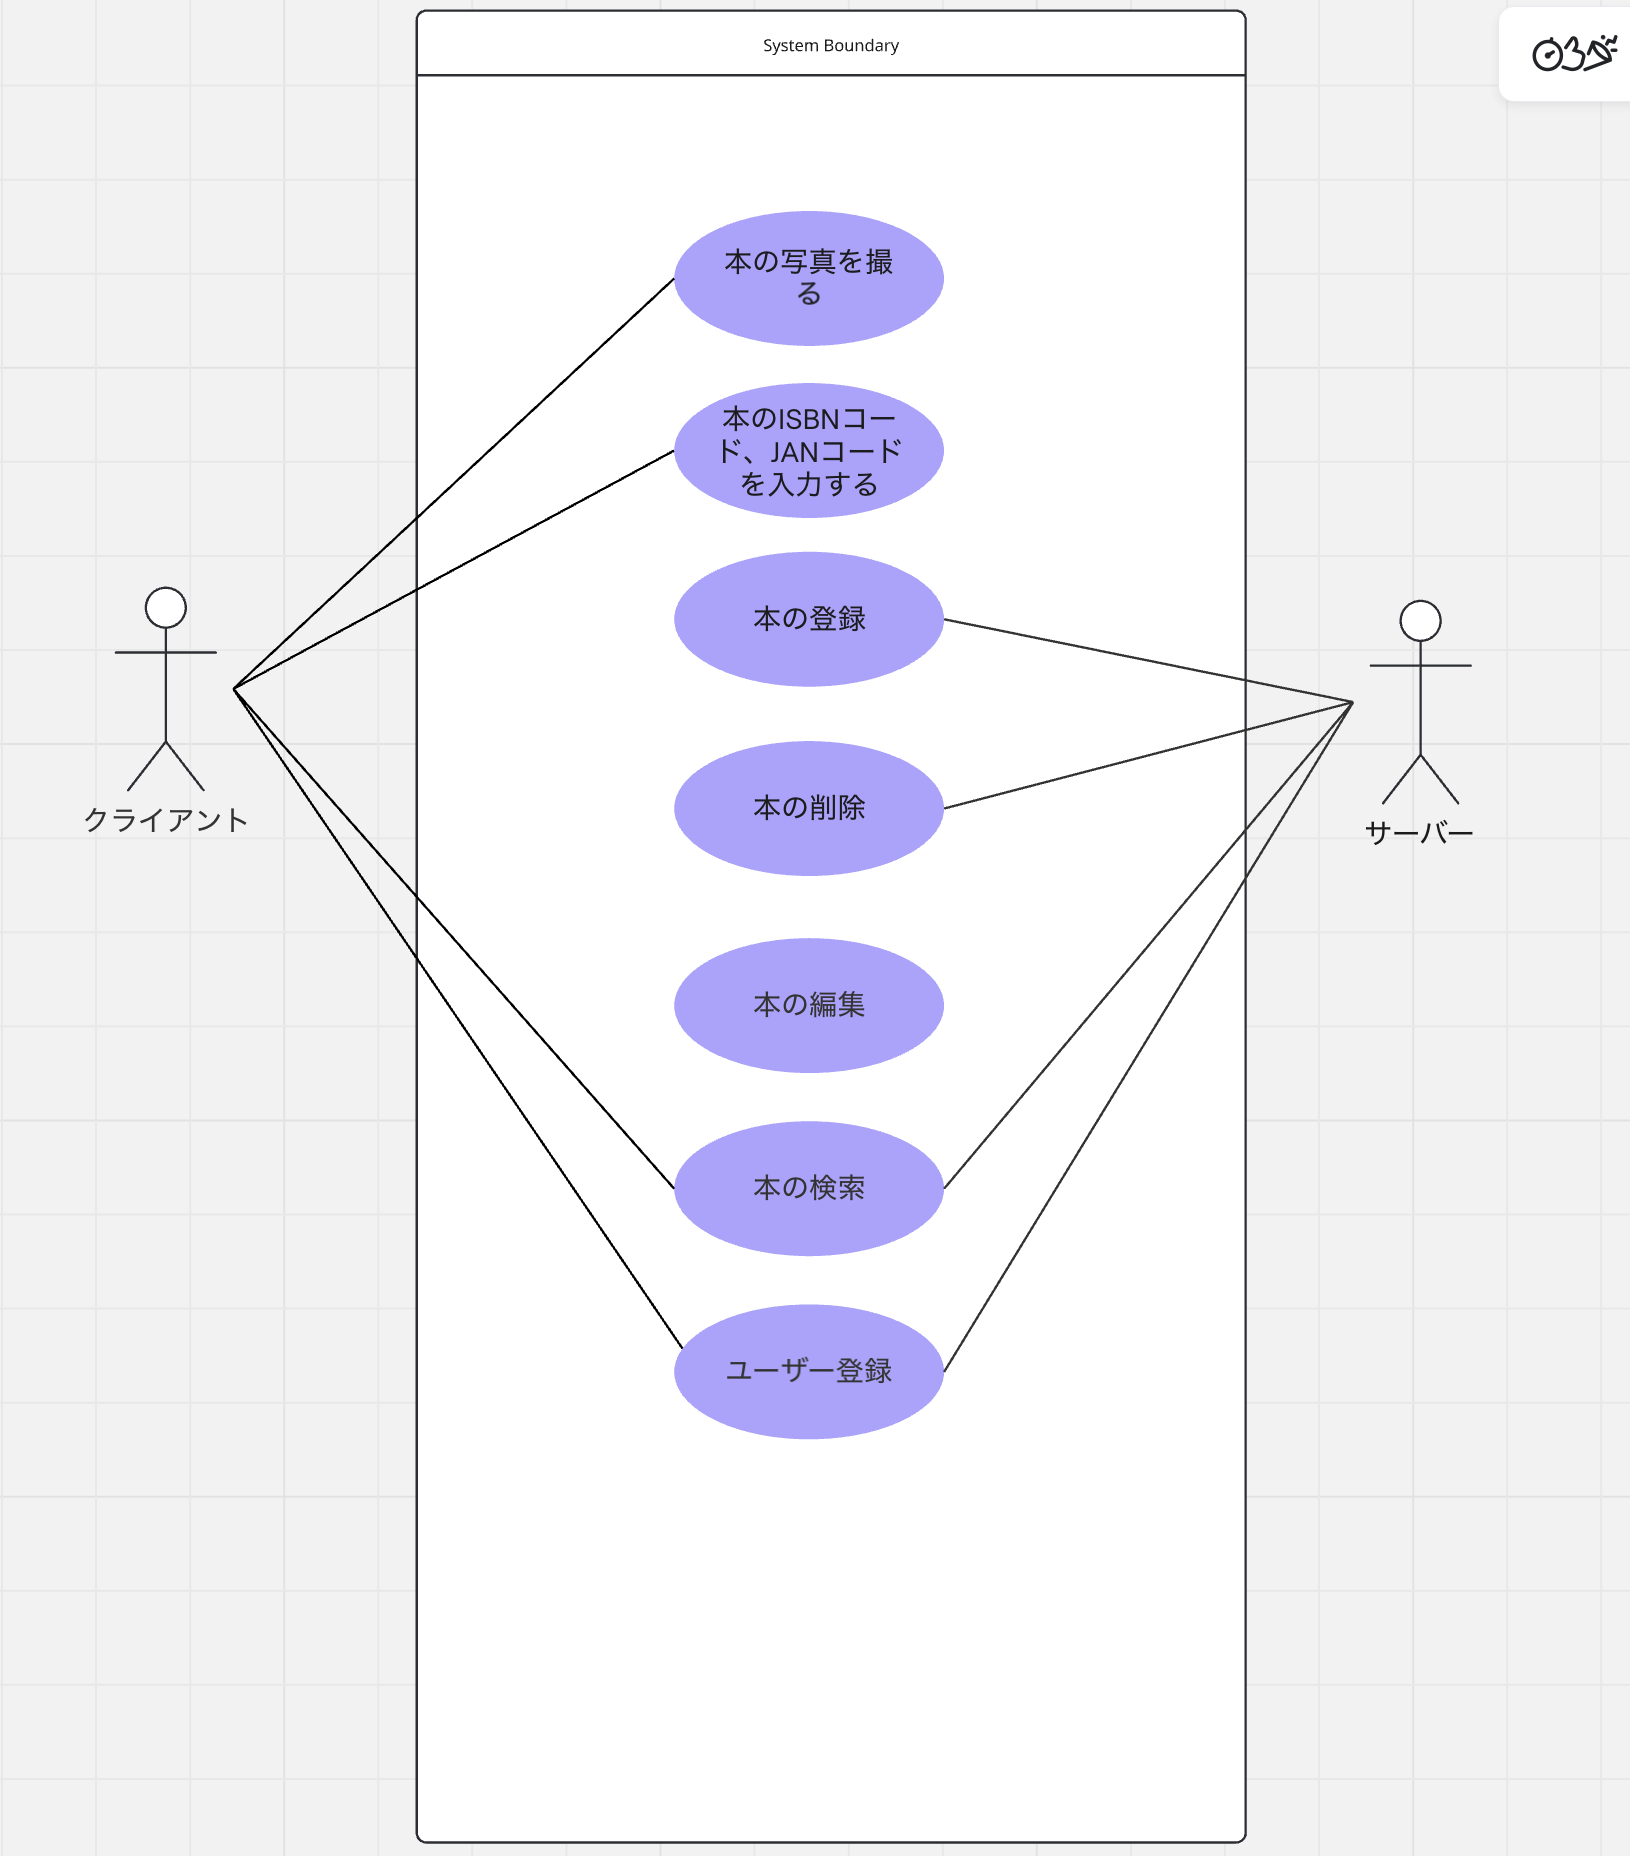
\includegraphics[width=80mm]{usecase.png}
\label{fig:func}
\end{figure}

この図は、ユーザー(クライアント)がシステムに対して行う操作と、それに伴うサーバーの役割を示しています。機能は大きく「本の登録」「登録後の本管理」「ユーザー管理」の3つの流れに分けられます。
\begin{itemize}
	 \item \textbf{1. 本の登録フロー} 
	ユーザーが新しい本を本棚に登録するまでの一連の流れです。

	\begin{itemize}
    		\item \textbf{本の特定(クライアント側の操作):}
    	まず、クライアント(ユーザー)が登録したい本を特定するための操作を行います。
    		\begin{itemize}
        			\item \textbf{本の写真を撮る:} スマートフォンのカメラなどで本の表紙を撮影します。
        			\item \textbf{本のISBNコード、JANコードを入力する:} 書籍の裏表紙などにあるバーコード情報を手動で入力します。
    		\end{itemize}
    	\item \textbf{本の登録(クライアントからサーバーへの依頼):}
    上記のいずれかの方法で本が特定されると、クライアントは\textbf{「本の登録」}を実行します。この操作は、特定された書籍情報を\textbf{サーバー}に送信し、データベースへの保存を依頼する役割を持ちます。
	\end{itemize}
	\item \textbf{2. 登録後の本管理} 
	サーバーに登録された本に対して、クライアントが行う操作です。これらの操作はすべてサーバー上のデータにアクセスする必要があります。

	\begin{itemize}
    		\item \textbf{本の編集:} 登録済みの本に対して、感想を追加・修正します。クライアントからの依頼を受け、サーバーがデータを更新します。
    		\item \textbf{本の削除:} 本棚から不要な本を削除します。クライアントからの依頼を受け、サーバーがデータを削除します。
    		\item \textbf{本の検索:} 登録されている膨大な本の中から、目的の本を探します。クライアントが入力した検索条件を元に、サーバーが該当するデータを返します。
	\end{itemize}
\end{itemize}
%---------------------------------------------------------------------------------------------------------------------------------------------------------------------------------------------------------------------------------------------------------------------------------
\clearpage
\section{詳細設計書}

\subsection{開発環境・ツール}
\begin{itemize}
  \item 使用する言語
  \begin{itemize}
    \item フロントエンド\\
    HTML(Jinja2), CSS
    \item バックエンド\\
    Python3
  \end{itemize}
  \item フレームワーク\\
  Flask
  \item 開発ツール\\
  VSC
  \item バージョン管理システム\\
  Git, GitHub
\end{itemize}

\subsection{システム構成}
ハードウェア構成は、ユーザーPCとサーバーPCの2つで構成されます。

ソフトウェア構成は、ユーザーPCのWebブラウザ、サーバーPCのWebサーバーで構成されます。データベースはSQLiteを使用するため、データベースサーバーは用意しません。

ネットワーク構成は、ユーザーPCがネットワークを介してサーバーPCにアクセスする形になります。

フロントエンドとバックエンドの構成図を次ページに掲載します。
\clearpage
\begin{figure}[htbp]
\centering
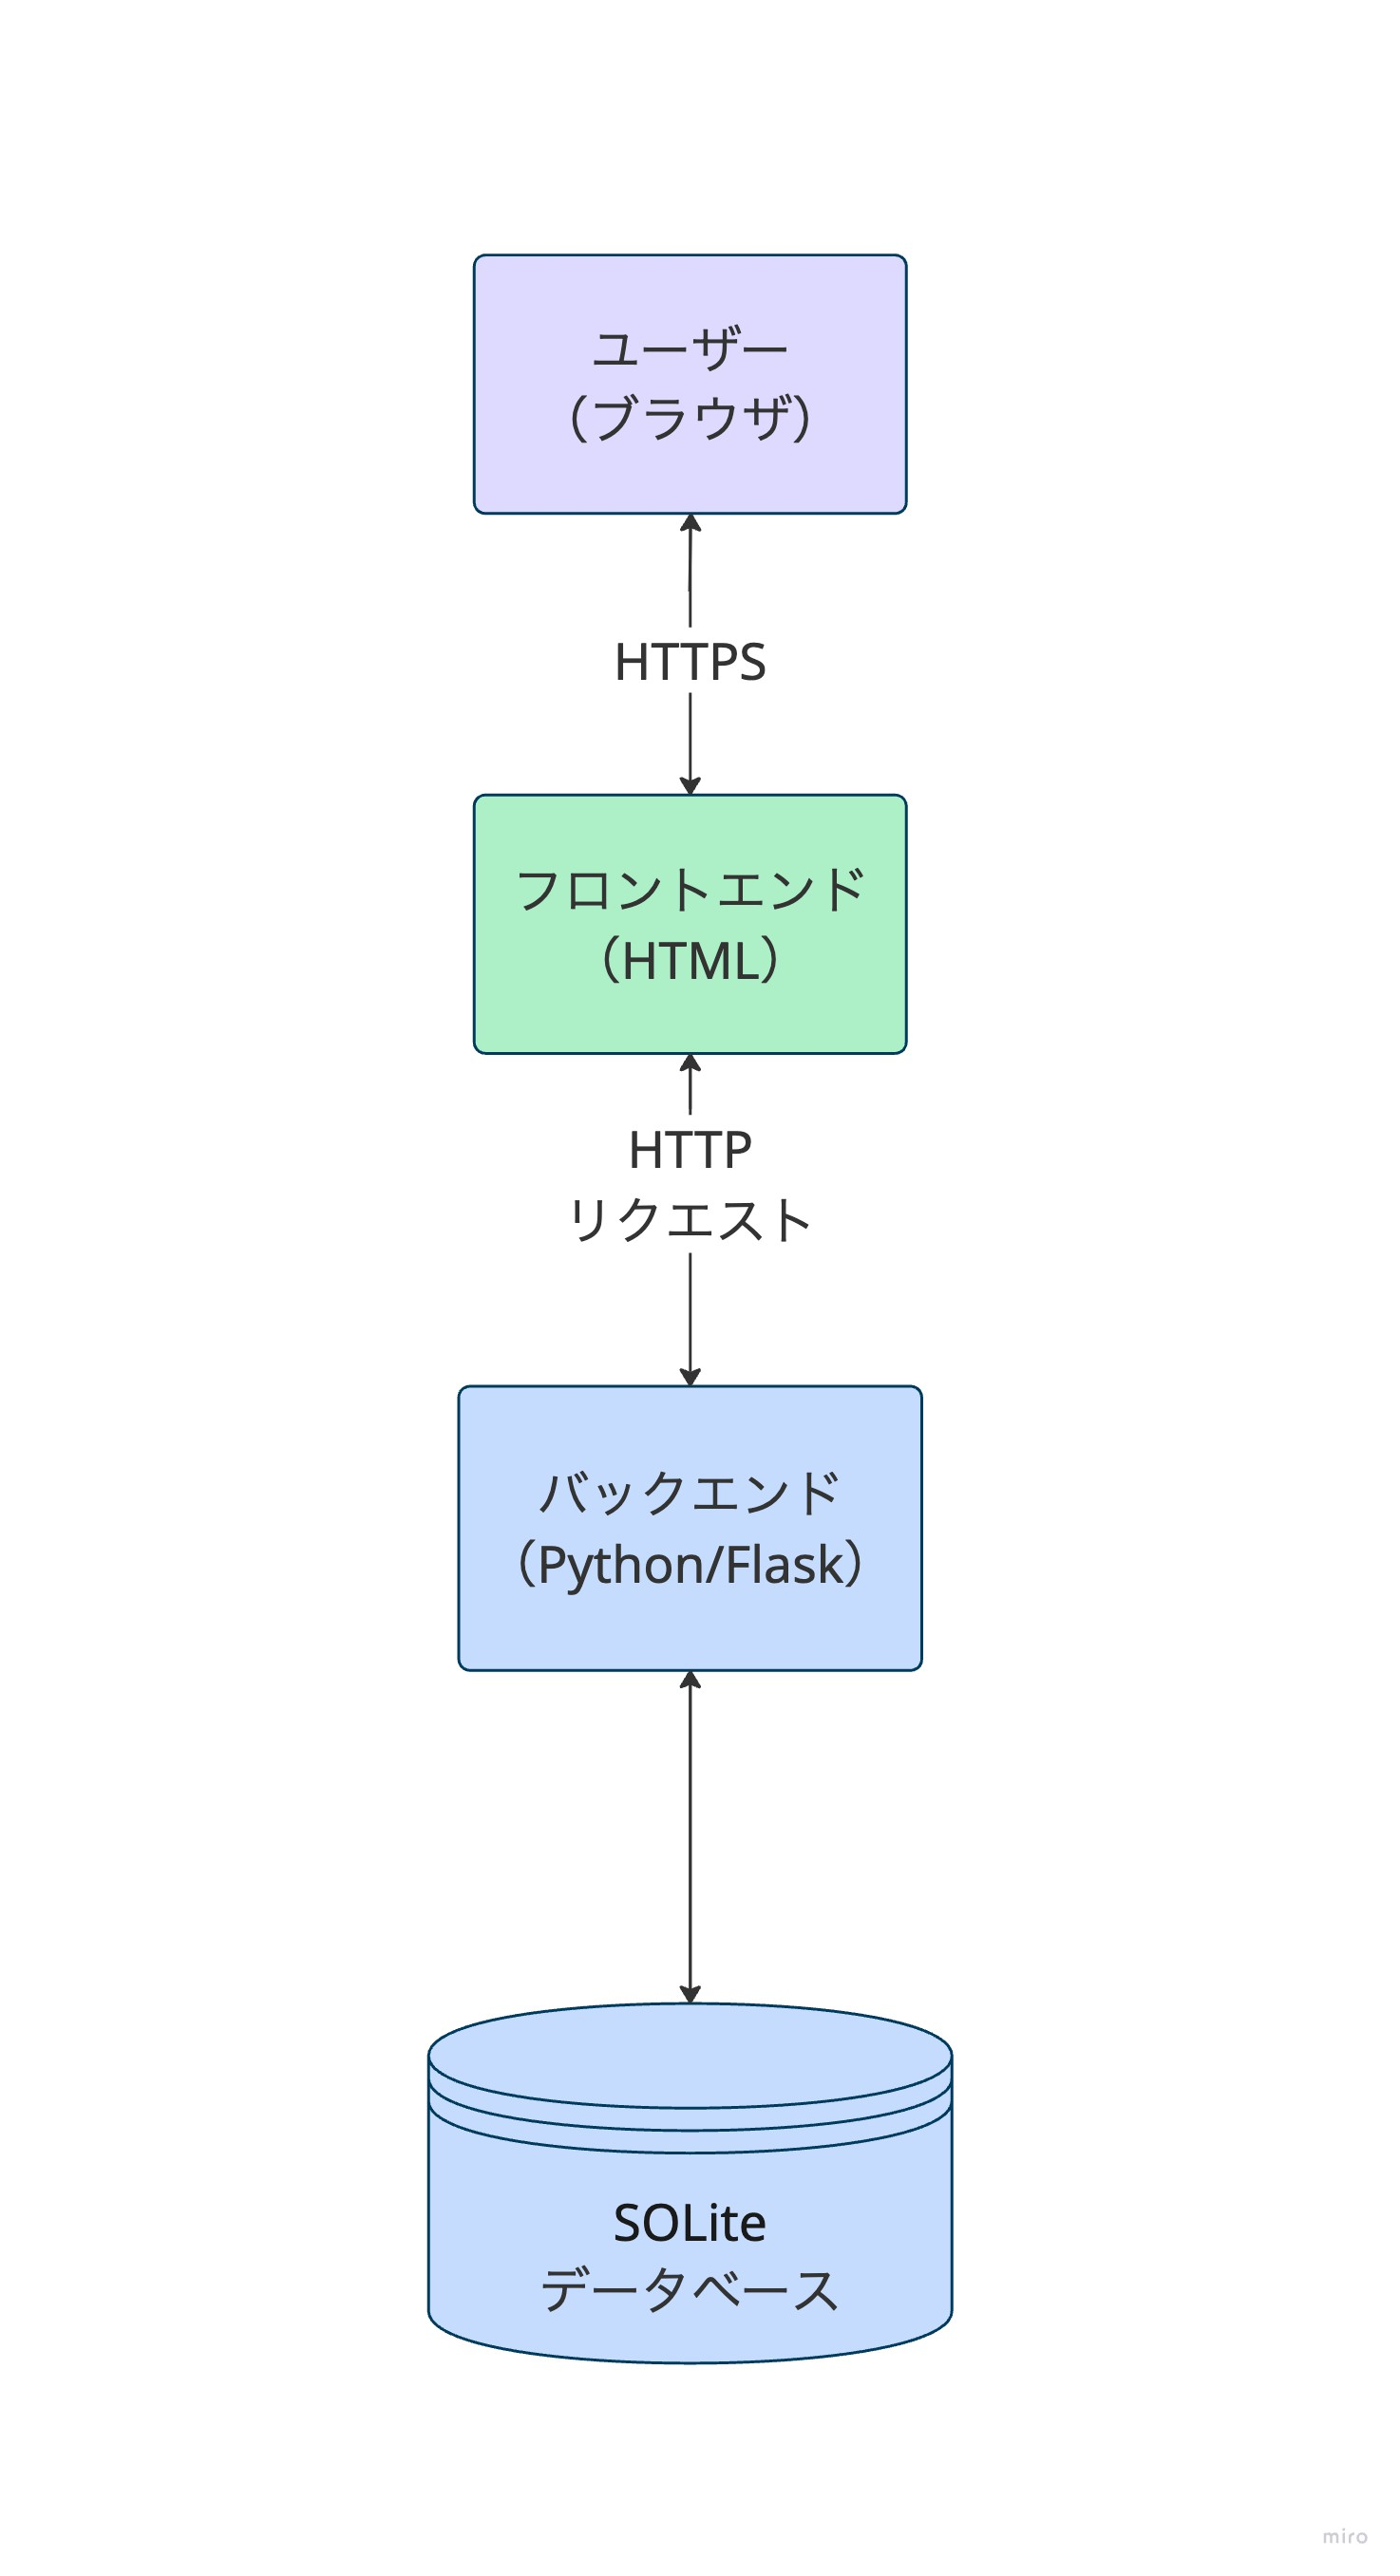
\includegraphics[width=70mm]{systemStructure.jpg}
\caption{システム構成図}
\label{fig:func}
\end{figure}

\subsection{データベース設計}
\subsubsection{ブックテーブル(book)}

ブックテーブルの主キーは'book\_id'で、本の一意な識別子です。IDの被りを防ぐため、AUTO\_INCREMENTも制約として設定しています。画像は'img'カラムに保存され、データ型はBLOBを使用し、バイナリデータで画像を保存します。'add\_date'は本の追加日時を記録するためのDATETIME型で、デフォルト値は現在日時に設定しています。その他のカラムは、書籍のタイトル、著者、出版社、ISBN、ジャンル、評価、感想を保存するためのVARCHAR型で、それぞれ適切な長さを設定し、NOT NULL制約を付けています。

\begin{table}[htbp]
  \centering
  \begin{tabular}{|l|l|>{\centering\arraybackslash}m{4cm}|>{\centering\arraybackslash}m{3cm}|}
    \hline
    \textbf{カラム名} & \textbf{データ型} & \textbf{制約} & \textbf{説明} \\
    \hline\hline
    book\_id & BIGINT & PRIMARY KEY, AUTO\_INCREMENT & 本の識別子 \\
    \hline
    img & BLOB & NOTNULL & 本の表紙、ページ \\
    \hline
    name & VARCHAR(255) & NOTNULL & 本のタイトル \\
    \hline
    author & VARCHAR(50) & NOTNULL & 本の著者 \\
    \hline
    add\_date & TIMESTAMP & NOTNULL, DEFAULT, CURRENT\_TIMESTAMP & 本の追加日 \\
    \hline
    code & VARCHAR(14) & NOTNULL & ISBNコード \\
    \hline
    memo & VARCHAR(511) & NOTNULL & 本の感想等自由記述(任意) \\
    \hline
    tag & VARCHAR(10) & NOTNULL & 本のタグ(任意) \\
    \hline
    message & VARCHAR(255) & NOTNULL & 完了メッセージ等の管理 \\
    \hline
  \end{tabular}
  \caption{ブックテーブル(book)}
  \label{tab:booktable}
\end{table}

\subsubsection{本棚テーブル(shelf)}
本棚テーブルの主キーは'shelf\_id'で、本棚の一意な識別子です。'shelf\_name'は本棚の名前を保存するためのVARCHAR型で、NOT NULL制約を付けています。外部キーとしてbook\_idを設定し、ブックテーブルのbook\_idと関連付けています。これにより、本棚に登録されている本の情報を参照できます。
\begin{table}[htbp]
  \centering
  \begin{tabular}{|l|l|>{\centering\arraybackslash}m{4cm}|>{\centering\arraybackslash}m{3cm}|}
    \hline
    \textbf{カラム名} & \textbf{データ型} & \textbf{制約} & \textbf{説明} \\
    \hline\hline
    shelf\_id & BIGINT & NOT NULL & 本棚の識別子 \\
    \hline
    book\_id & BIGINT & NOT NULL & 本の識別子 \\
    \hline
  \end{tabular}
  \caption{本棚テーブル(shelf)}
  \label{tab:shelftable}
\end{table}

\clearpage
\subsection{各機能の処理フロー}
\subsubsection{書籍一覧表示}
ユーザーがはじめに行う操作は、ホームボタンを押すことです。それにより、アプリ側はトップページに遷移し、本棚情報をデータベースから取得します。取得した本棚情報から、本棚の画像や名前をレンダリングします。
ユーザーがはじめに行う操作は、ホームボタンを押すことです。それにより、アプリ側はトップページに遷移し、本棚情報をデータベースから取得します。取得した本棚情報から、本棚の画像や名前をレンダリングします。
\begin{figure}[htbp]
  \centering
  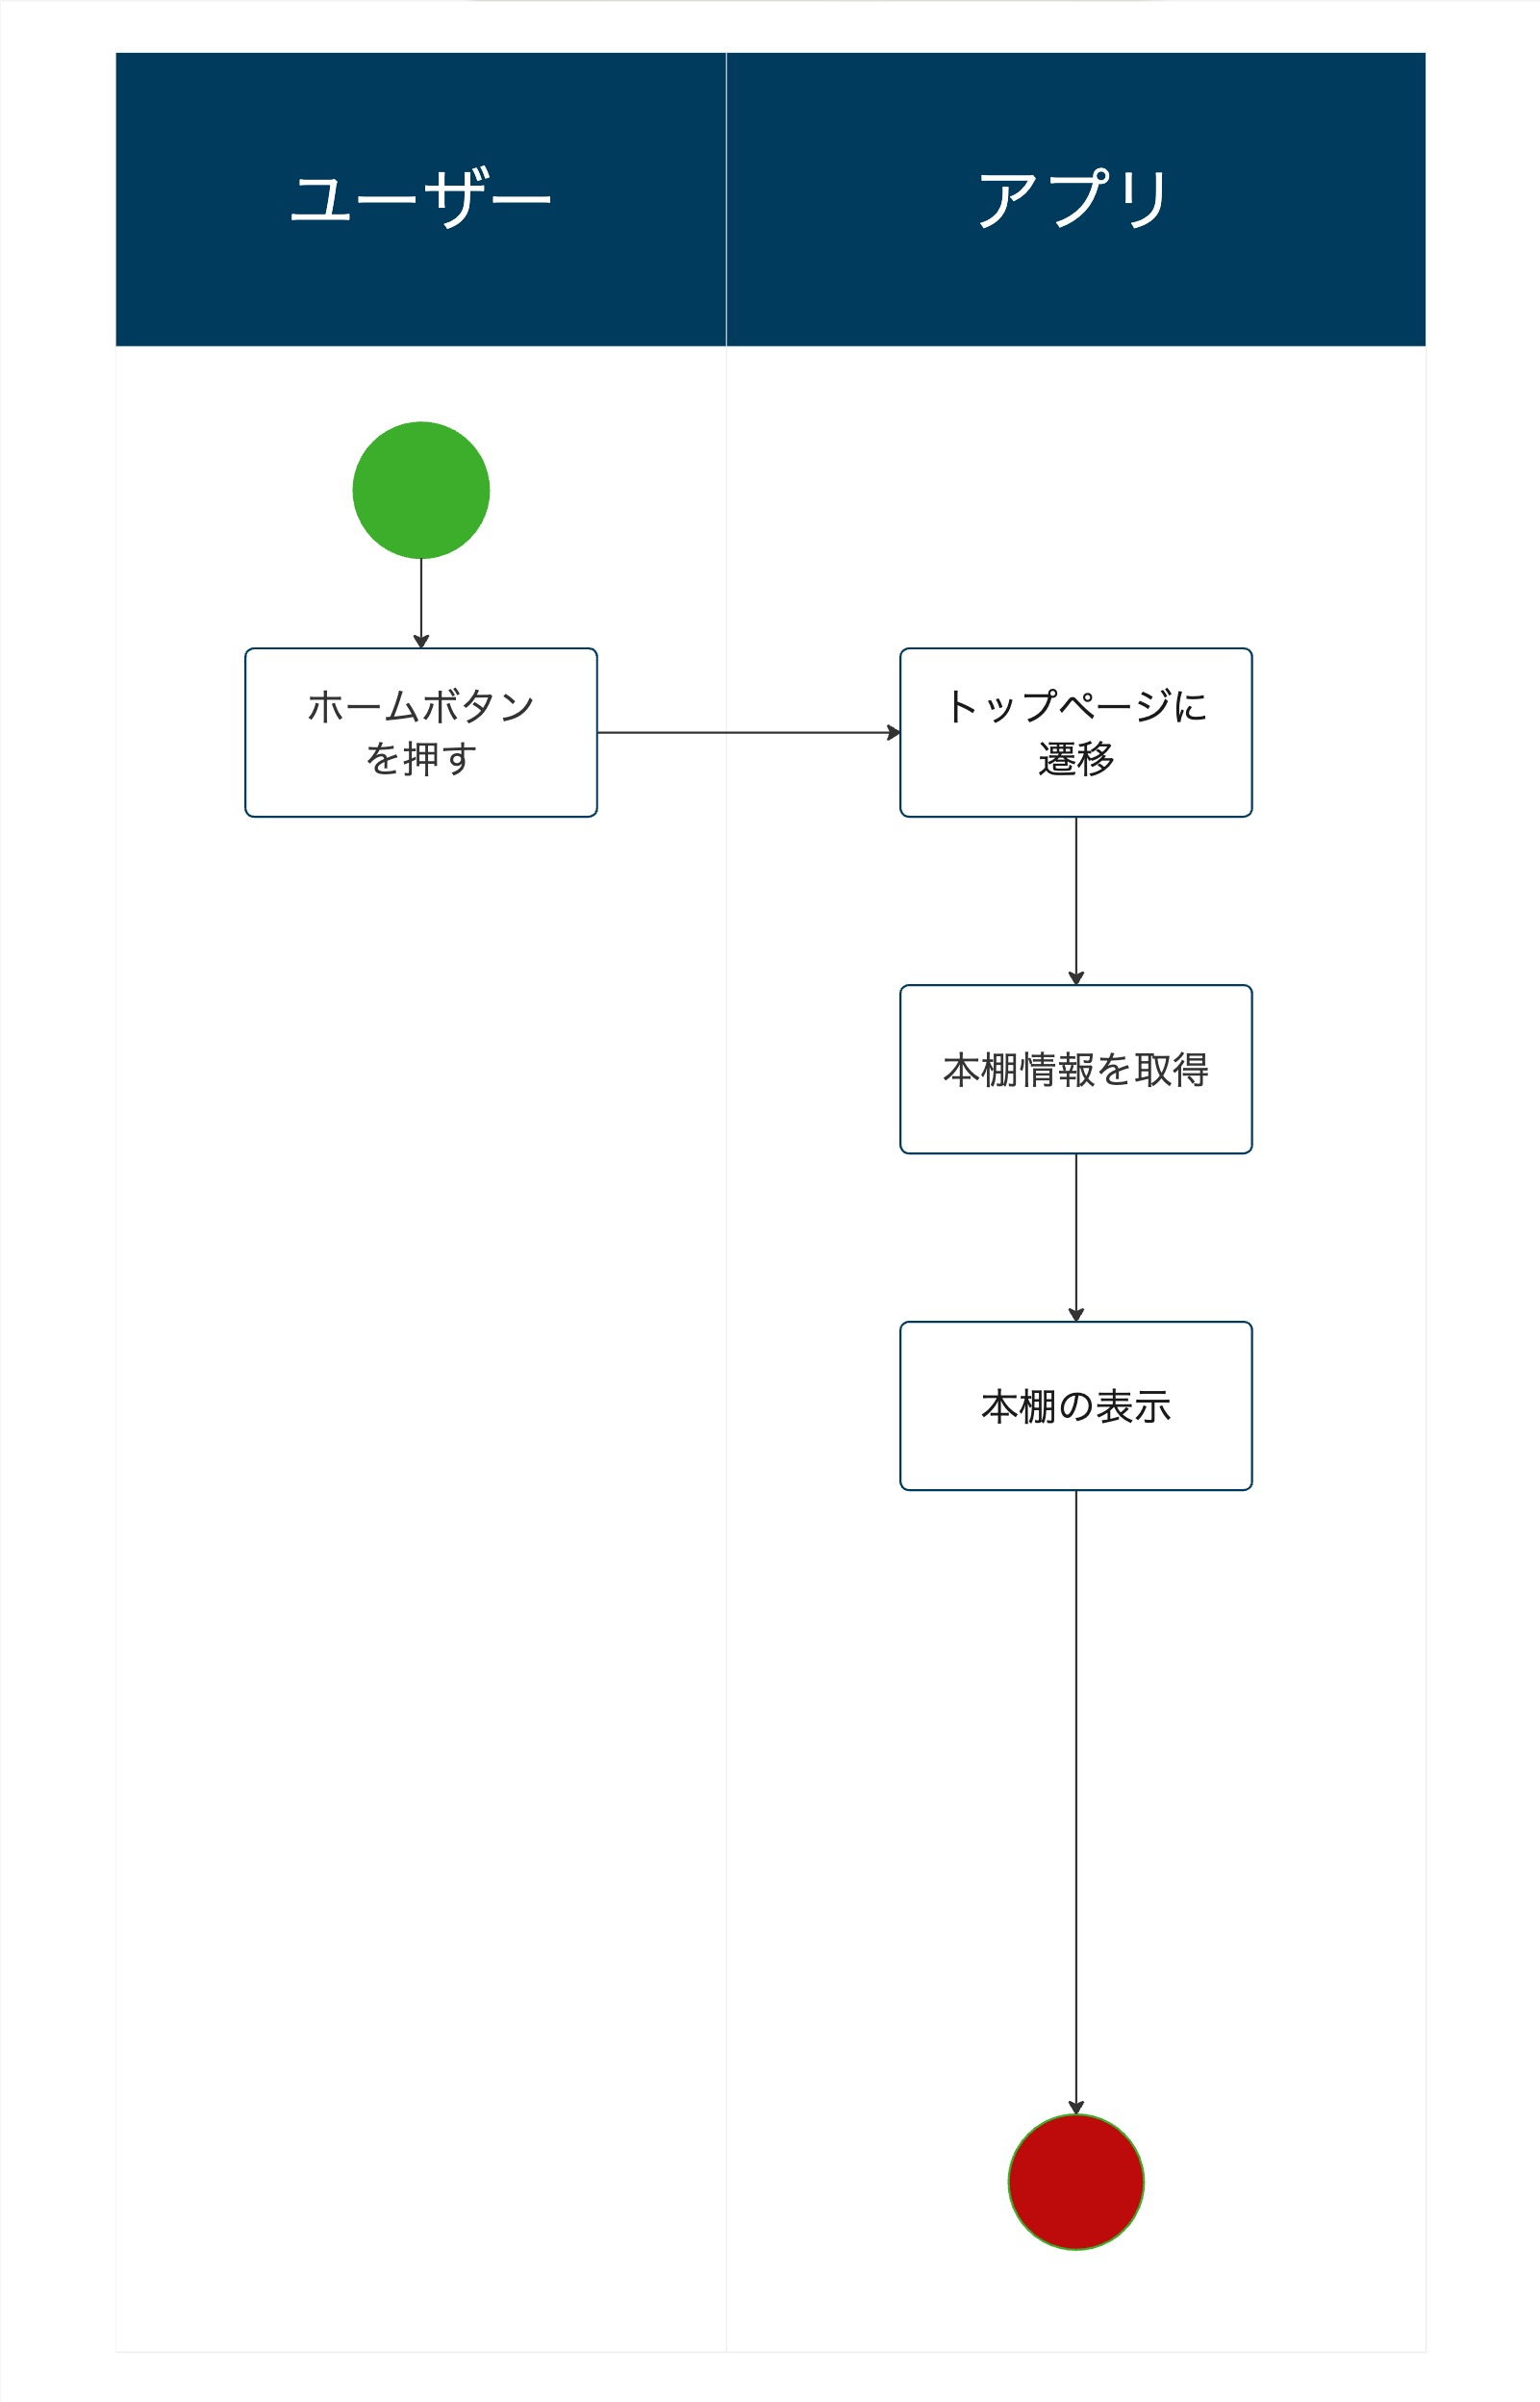
\includegraphics[width=90mm]{flow-ichiran.jpg}
  \label{fig:func}
\end{figure}

\clearpage
\subsubsection{書籍登録}

ユーザーが書籍の登録を要求する、すなわち登録ボタンを押すと、アプリ側で登録フォームを表示し、ユーザーに各種情報の入力を求めます。ユーザーが必要な情報を入力し、登録ボタンを押すと、アプリ側はその情報がフォームの入力規則に従っているかを検証します。検証が成功すると、アプリ側はデータベースに書籍情報を登録し、検証が失敗すると、エラーメッセージを表示します。登録が成功すると、ユーザーは登録完了のメッセージを受け取り、トップページにリダイレクトされます。
\begin{figure}[h]
\centering
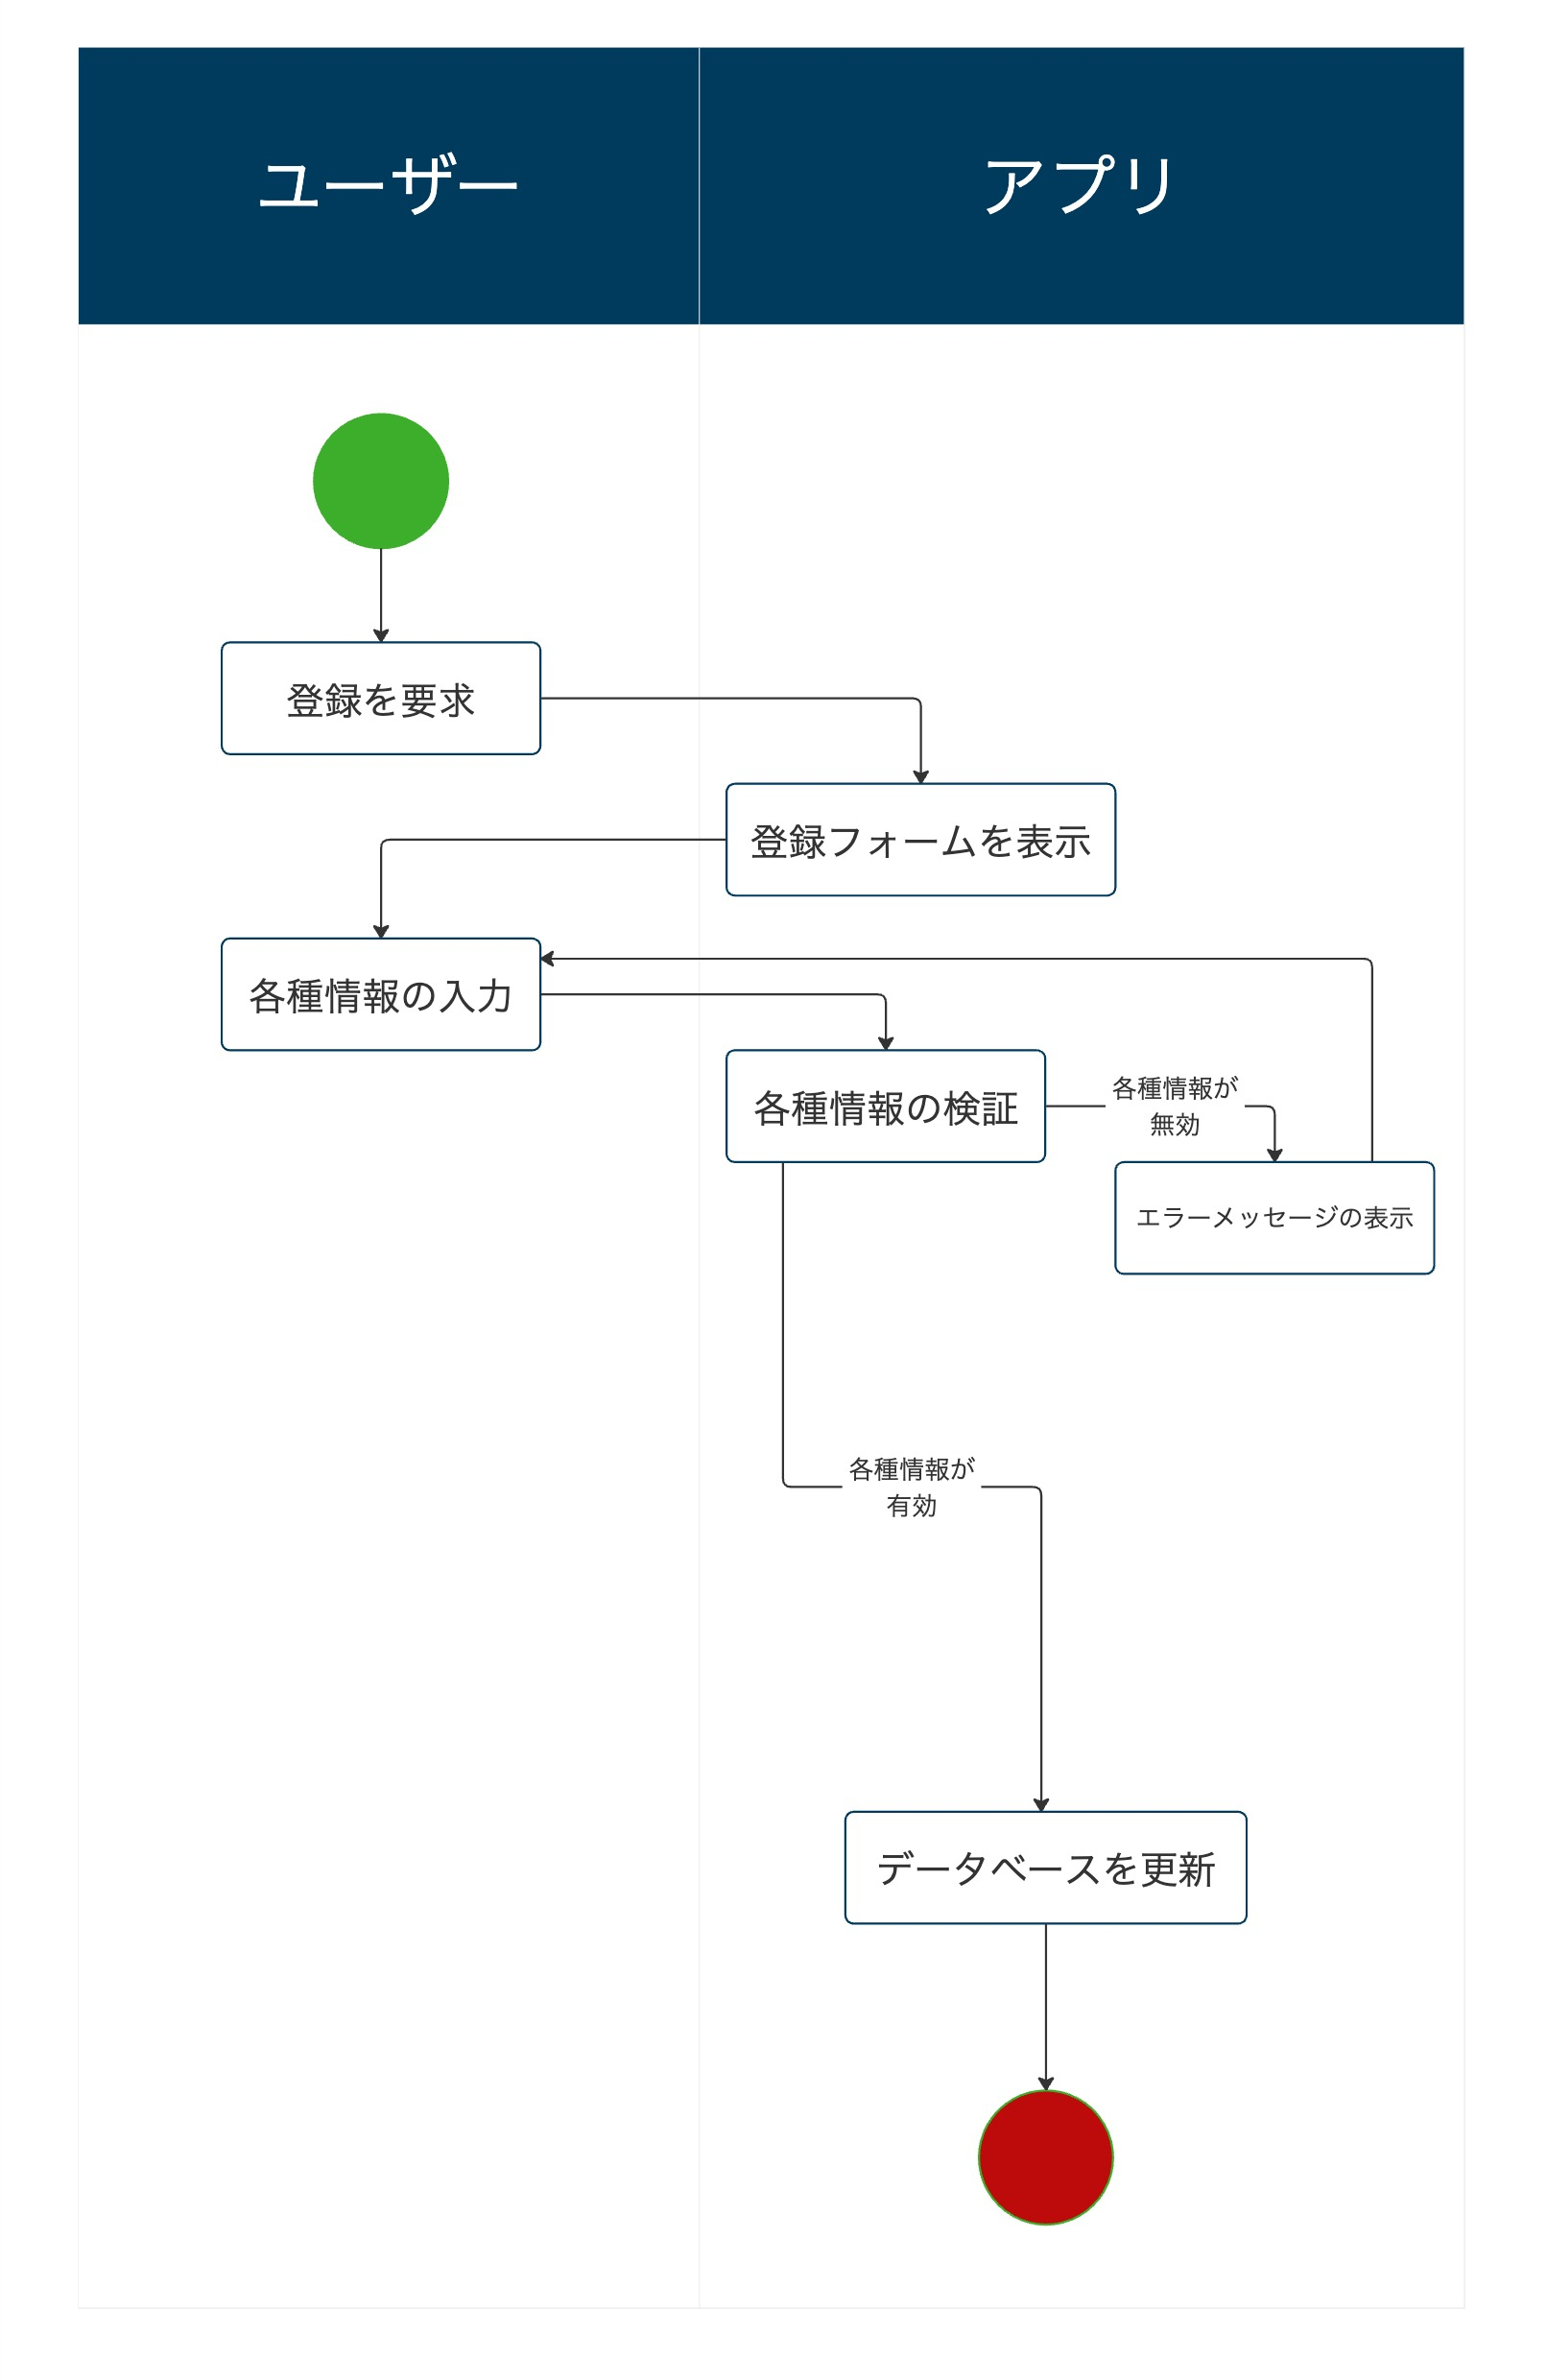
\includegraphics[width=90mm]{flow-touroku.jpg}
\label{fig:func}
\end{figure}

\clearpage
\subsubsection{書籍編集}
ユーザーが本のページを開き、書籍編集を要求、すなわち編集ボタンを押すと、アプリは本の詳細を編集可能な状態にし、各種内容を編集するフォームを出力します。ユーザーは感想等の自由記述、タグの設定が可能で、アプリ側でタグがすでに存在するなら、書籍情報がタグに紐づけられます。タグが存在しない場合は、編集内容を登録し、アプリ側は新しいタグを作成します。ユーザーが編集内容を保存すると、アプリ側はデータベースに変更を上書き更新し、更新完了のメッセージを表示します。これにより、ユーザーは本の詳細情報を自由に編集できるようになります。
\begin{figure}[h]
\centering
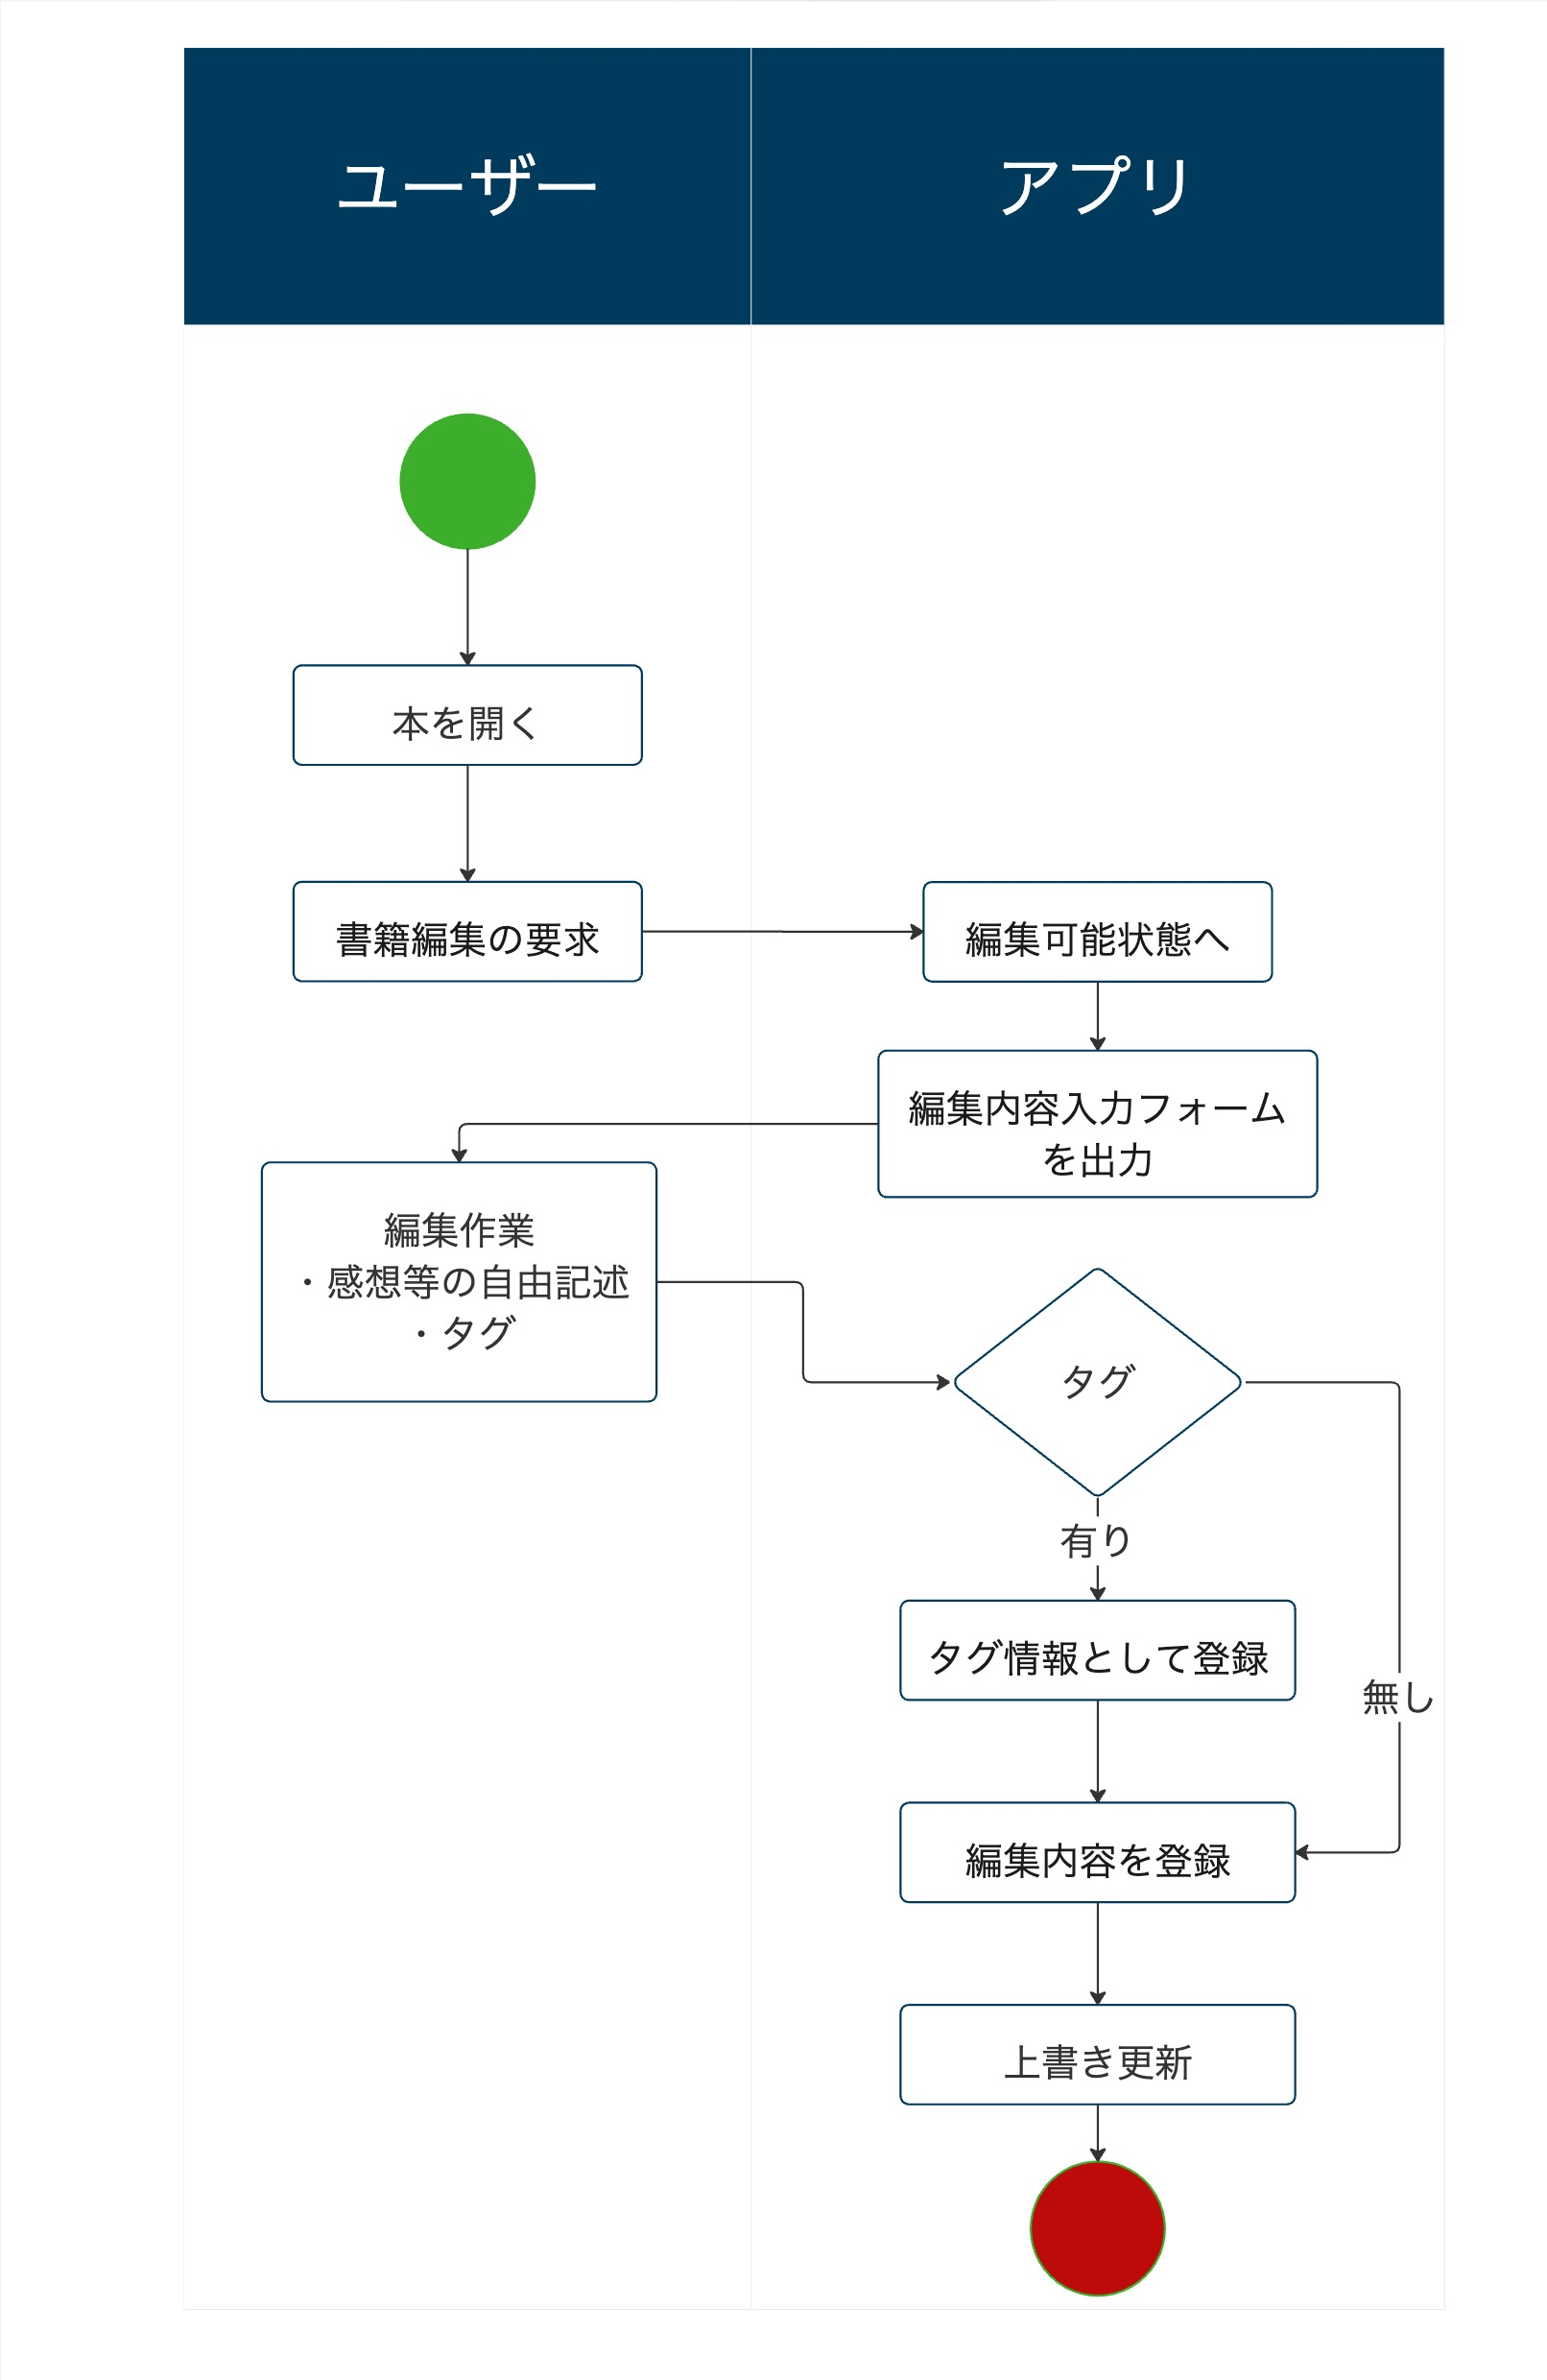
\includegraphics[width=100mm]{flow-henshu.jpg}
\label{fig:func}
\end{figure}

\section{グループでの分担内容と貢献度、MVP}%----------------------------------------------------------------------------------------------

\subsection{詳細設計書におけるグループでの分担内容と貢献度}
\begin{itemize}
    \item \textbf{245429H 末吉 良多(30\%)}開発環境・ツールと書籍一覧表示フローを作成。
    \item \textbf{245745J 知念 拓弥(40\%)}システム構成図と書籍登録フローを作成。とりまとめ。
    \item \textbf{245704B 武嶋 優海(30\%)}データベース設計と書籍編集フローを作成。
\end{itemize}

\textbf{MVP : 245745J 知念拓弥}

\end{document}